

\chapter{Project Overview}
\ifpdf
    \graphicspath{{chapter_1/figures/PNG/}{chapter_1/figures/PDF/}{chapter_1/figures/}}
\else
    \graphicspath{{chapter_1/figures/EPS/}{chapter_1/figures/}}
\fi
Anticancer is a method which prevent the development of cancer. Anticancer is basically used for cancer treatment.

\section{Introduction}
Cancer, the emperor of all maladies \cite{mukherjee2010emperor}, is the mostly deadly of all diseases and has been spreading as an epidemic for the last few decades. Due to advances in radiation and chemotherapy, nowadays cancer is being treated in most of the cases. However, most of these treatments come with side effects that damages normal cells. Thus anticancer peptides (ACP) have emerged as more effective means to treat cancer due to high precision \cite{otvos2008peptide}. ACPs are short sequences of amino acids, generally of length varying from 5 to 30 monomers. However, the discovery of anticancer peptides using \textit{in vitro} methods is expensive and time consuming. 


Prediction of many biological entities related to genomics, transcriptomics and proteomics have been formulated as supervised learning problem and hence many machine learning methods are applied to solve them in recent times \cite{chou2011some,jani2018irecspot,rayhan2018cfsboost,rahman2018ipromoter,chowdhury2017idnaprot}. Similar to those problems, the prediction of anticancer peptides can be formulated as a binary classification task where given an unknown peptide sequence the task of the predictor is to predict whether that is an anticancer peptide or not based on a dataset collected from already verified instances of anticancer peptides. Several methods in the literature are found that address the anticancer peptide prediction as a binary classification task \cite{tyagi2013silico,vijayakumar2015acpp,hajisharifi2014predicting,chen2016iacp,wei2018acpred}. 


Most of these methods are dependent on derived features (structural and evolutionary) that are computationally expensive to generate. Many ensemble methods like Adaboost \cite{rayhan2018cfsboost} and Random Forest \cite{jani2018irecspot} are applied to solve these problems where single classifiers fails to produce good results. Random Forest classifier randomly selects features and builds ensemble of decision trees. On the other hand, Adaboost  learns classifiers in an iterative manner by adjusting weights of the misclassified instances.

\section{Basic Biological Entities}
\begin{wrapfigure}{r}{0.35\textwidth}
\centering
    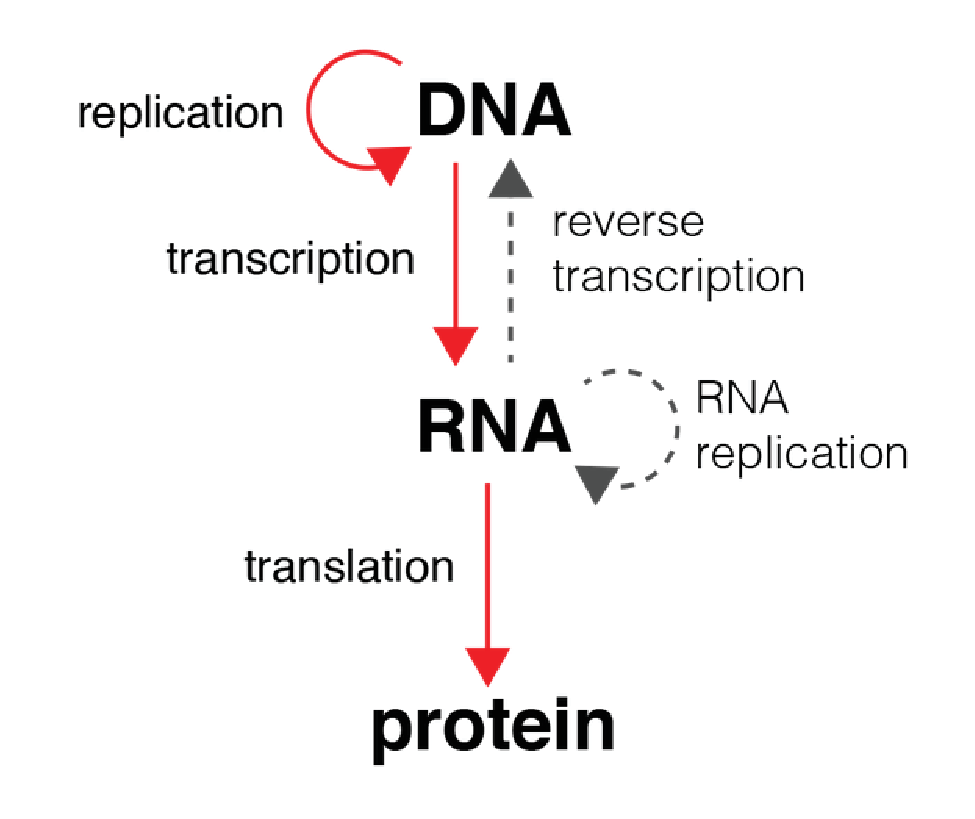
\includegraphics[width=0.35\textwidth]{dna.eps}
  %\label{fig:te}
  %\caption*{\scriptsize Source:\url{https://www.quora.com/What-is-the-central-dogma-of-molecular-biology-Is-it-true}}
  \caption{Central Dogma of Molecular Biology}\cite{Anderson03}
  
\end{wrapfigure}
\leavevmode

Biological entities means details about life and living beings. Every life and living being considered as individual organisms. For example two human may affect each other but their bodies are independent to each other. They have their own energy, unique set of genes and body metabolism. If we consider bacteria they are also considered as distinct organism, even if they are living inside us or inside our food.
%\begin{wrapfigure}{l}{0.19\textwidth}
%\centering
    %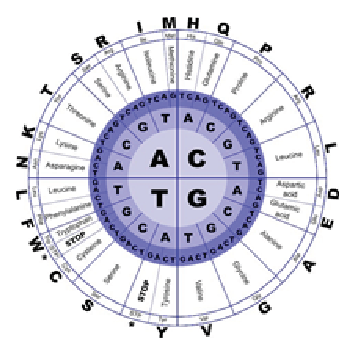
\includegraphics[width=0.19\textwidth]{dna2.eps}
  %\caption{Genetic code}
%\end{wrapfigure}
%\leavevmode

In most organisms the genetic information are stored in DNA (Deoxyribonucleic acid). First, By dividing cells DNA double strands became single and cells have completely new genomes. This process is known replication. Then RNA (Ribonucleic acid) is transcribed from DNA, and the protein is translated from RNA. The cell life is described from amino acid, which contains proteins.


\subsection{Pros and Cons}
Biological entity plays a vital role in our life. Predicting attributes or functionality will be helpful for biologist and clinical researcher.
But we need large, balanced data set and strong prediction algorithm to predict or the result may become harmful for human being.

\subsection{Tools}
Table following table shows the technical tools \& programming languages which we will be used for this tool.
\begin{table}[htbp]
\caption[Tools]{Name of tools \& languages.}
\centering
\footnotesize
\begin{tabular}{|c|c|c|} \hline
\bf No. & \bf Technical Tools & \bf Programming Languages \\\hline
1. & Latex & Python  \\\hline
2. & Anaconda & PHP \\\hline
3. & PyCharm & JavaScript \\\hline
4. & Notepad++ & Mysql  \\\hline
\end{tabular}
%\label{training_testing_examples_KDD99}
\end{table}

%\includegraphics[width=\textwidth]{tools}

\section{Motivation}
Biological entities are the source of the information of cell. Predicting the attribute or functionality is helpful for biologist and clinical researcher. Especially to find the cure of cancer and diabetes or to find new diseases or help to find reasons of that diseases. By using machine learning algorithms, new features, and methods for detection and prediction will be invented. That will play a vital role on our social and economics especially human life.

\section{Our Project}
We are working with biological entities to predict attributes based on biological entities. And also develop a web based tool which will be able to predict results from given protein sequence.

\subsection{Description of the Project}
The idea behind the project is to develop a web based tool that relies on a sequence which will be able to detect biological entity. In this project, we propose a new ensemble classifier for anticancer peptide prediction. Our ensemble classifier divides the feature space into subspaces and weak classifiers are learned on the subspaces. The ensemble classifier then provides a majority voting classification based on the predictions given by each weak classifiers. We have used simple sequence based features and divided them into three groups. Each group was then used to be learnt using weak classifiers. Tested on a standard benchmark dataset for anticancer peptides, our method significantly outperforms most other state-of-the-art methods for anticancer peptide prediction. Our method is different from Random Forest and Adaboost in the way it divides the feature space and learns the single weak classifiers.


\subsection{Difficulties}
First challenge is to collect balanced dataset, after collecting data set, feature collection is also a challenging task. Because there's a need to find out more features which will help to predict attributes with more accuracy using different algorithms. At last development of the tool with created model will also be challenging for us.

\section{Methodology}
First we formulate the problem, then we collect data according to our problem formulation. Then we extract some feature from the data set and use some classifier algorithm to predict biological entities from the data, then we validate it and create a model for our website tool. At last we will finish our tool development using the created model.

\figuremacroW{Methedology.eps}{Methodology}{Steps of methodology}{0.8}


\section{Summary}
In this chapter we know about the basics of biological entities, methods which we are following, pros and cons of predicting biological entities, Tools which we are using, our proposed project idea, difficulties which we may face to complete our project and motivation of making this project. The thesis is organized as : Chapter \ref{Related Work} provides related works, Chapter \ref{Methods} presents methods, Chapter \ref{Impact} discusses about the impact, Chapter \ref{Result} presents the result and Chapter \ref{Conclusion} presents conclusion.

